Cette section est une application de la méthode de Newton-Raphson à une fonction spécifique afin de déterminer toutes les racines réelles et complexes d'un polynôme.

\subsection{Explication de l'algorithme}

L'algorithme de Bairstow sert à déterminer toutes les racines d'un polynome P de degré n. Dans un premier temps, cette méthode consiste à calculer tous les facteurs quadratiques $X^{2} + BX + C$ de ce polynome. Dans un second temps, les racines de ces facteurs quadratiques sont calculées.

\bigskip

\indent On considère une fonction vectorielle F(B, C) définie de $\nbR^2$ vers $\nbR^2$ par $F(B, C) = (R, S)$. Les termes B et C sont les coefficients du polynome quadratique $X^{2} + BX + C$. Les termes R et S sont respectivement le coefficient de X et le terme constant du reste de la division de P(X) par $X^{2} + BX + C$.

\bigskip

\indent Trouver les zéros de  cette fonction F revient à déterminer $F(B, C) = (0, 0)$.
Cette équation est vérifiée lorsque que $X^{2} + BX + C$ divise exactement P(X). Les termes B et C sont donc calculés par la méthode de Newton-Raphson.

\bigskip

\indent Chaque zéro (B, C) de F correspond ainsi à un facteur quadratique de P(X), ce qui permet d'extraire deux racines (réelles ou complexes conjuguées) de P(X) sans avoir à manipuler directement des nombres complexes.

Les quatre dérivées partielles de la fonction vectorielle F sont $\frac{\partial R}{\partial B}$, $\frac{\partial R}{\partial C}$, $\frac{\partial S}{\partial B}$ et $\frac{\partial S}{\partial C}$.
\bigskip

\noindent Les dérivées partielles par rapport à C sont obtenues par les équations~\eqref{eq1}.

\begin{equation}
    \frac{\partial R}{\partial C} = -R_1 \hspace{1cm} et \hspace{1cm}
    \frac{\partial S}{\partial C} = -S_1
    \label{eq1}
\end{equation}

\noindent Les dérivées partielles par rapport à B sont elles données par les équations~\eqref{eq2}.

\begin{equation}
    \frac{\partial R}{\partial B} = BR_1 - S_1 \hspace{1cm} et \hspace{1cm}
    \frac{\partial S}{\partial B} = CR_1
    \label{eq2}
\end{equation}

\subsection{Applications de l'algorithme}

L'application de l'algorithme de Bairstow sur différents polynômes a permis d'analyser les
performances de ce dernier.

\begin{figure}[!h]
    \centering
    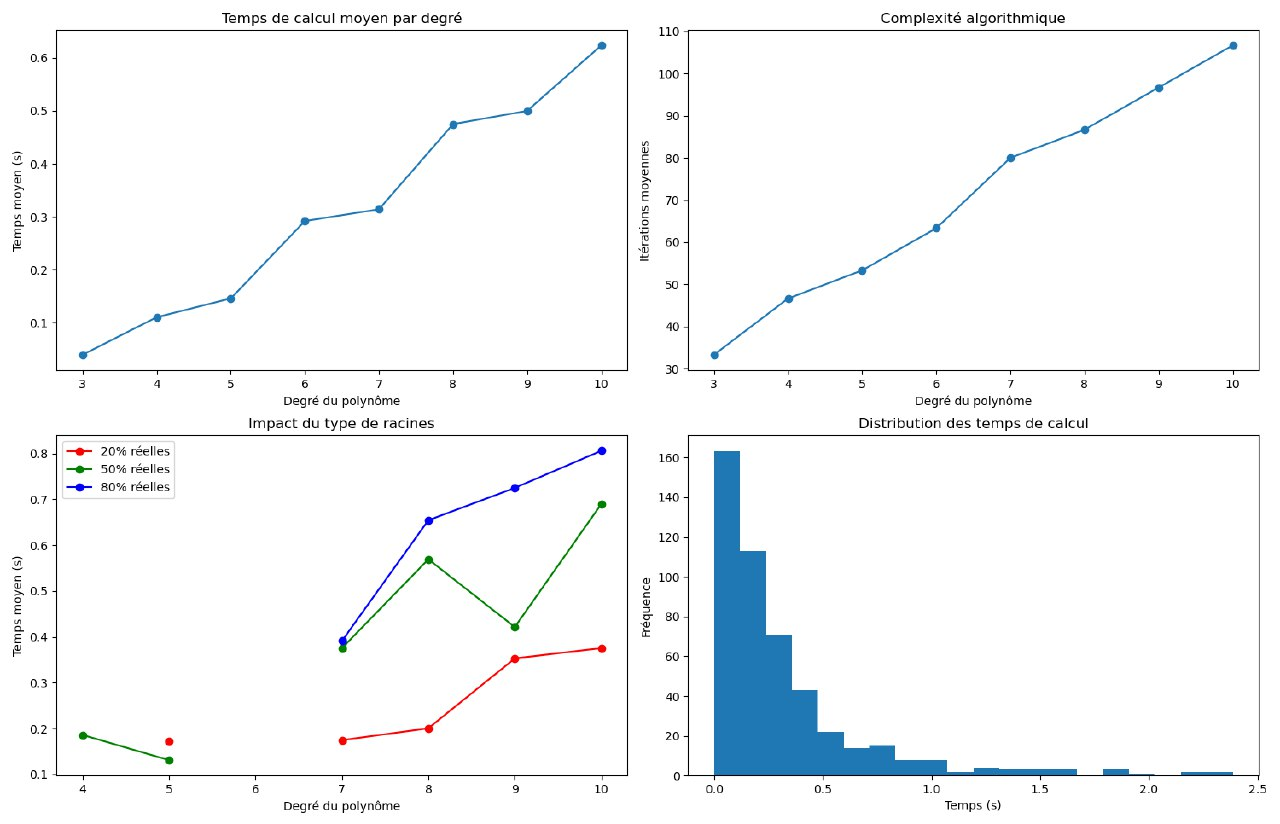
\includegraphics[width=0.90\textwidth]{graphs_bairstow.jpg} 
    \caption{Performances de l'algorithme de Bairstow}
    \label{fig:graph_bairstow} 
\end{figure}

\bigskip

Le graphique en haut à gauche de la figure~\ref{fig:graph_bairstow} indique que plus le degré du polynôme est élevé, plus 
le temps de calcul moyen augmente. Cela suggère que la complexité du calcul croît avec le degré du polynôme.\\

De même, le graphique en haut à droite de la figure~\ref{fig:graph_bairstow} montre une augmentation d'itérations avec le degré du
polynôme. Le temps de calcul est donc directement impacté.

\bigskip

Nous observons également d'après le graphique en bas à gauche de la figure~\ref{fig:graph_bairstow} que le temps de calcul moyen augmente avec le degré du polynôme quelle que soit la proportion
de racines réelles. De plus, l'algorithme prend plus de temps pour les polynômes avec plus de racines réelles.
Cela montre que l'algorithme de Bairstow est plus efficace pour les polynômes ayant principalement des racines
complexes.

\bigskip

La majorité des calculs de l'algorithme de Bairstow sont réalisés en un temps proche de 0 comme le montre
le graphique en bas à droite de la figure~\ref{fig:graph_bairstow}. Cependant, malgré l'efficacité de l'algorithme, il existe 
certains cas pour lesquels le temps de calcul est plus élevé. Cela peut être dû à des polynômes plus complexes
à résoudre.
